\documentclass[tikz,border=3mm]{standalone}
\begin{document}

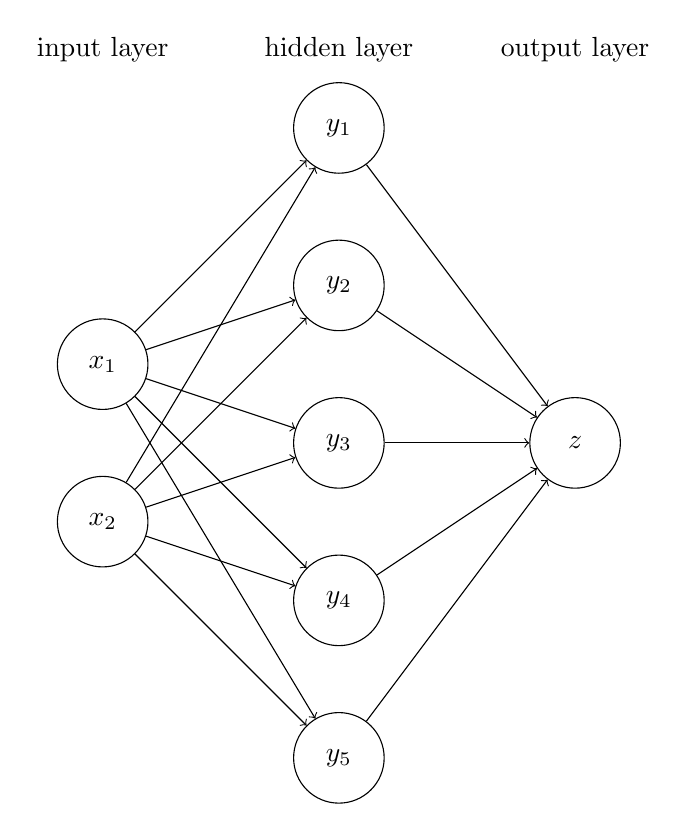
\begin{tikzpicture}
	\tikzstyle{node}=[draw,shape=circle,minimum size=1.15cm]

	\node[node](x1) at (0,2){$x_1$};
	\node[node](x2) at (0,0){$x_2$};

	\node[node](y1) at (3,5){$y_1$};
	\node[node](y2) at (3,3){$y_2$};
	\node[node](y3) at (3,1){$y_3$};
	\node[node](y4) at (3,-1){$y_4$};
	\node[node](y5) at (3,-3){$y_5$};
		
	\node[node](z) at (6,1){$z$};

	\draw[->] (x1) -- (y1);
	\draw[->] (x1) -- (y2);
    \draw[->] (x1) -- (y3);
	\draw[->] (x1) -- (y4);
	\draw[->] (x1) -- (y5);

	\draw[->] (x2) -- (y1);
	\draw[->] (x2) -- (y2);
    \draw[->] (x2) -- (y3);
	\draw[->] (x2) -- (y4);
	\draw[->] (x2) -- (y5);

	\draw[->] (y1) -- (z);
	\draw[->] (y2) -- (z);
	\draw[->] (y3) -- (z);
	\draw[->] (y4) -- (z);
	\draw[->] (y5) -- (z);
	
	\draw (0,6) node {input layer};
	\draw (3,6) node {hidden layer};
	\draw (6,6) node {output layer};
\end{tikzpicture}

\end{document}